% !TeX root = ../main.tex
\chapter{Theoretical background}
\label{chap:background}

Da qualche parte cita \cite{carosso2020novel}. \\~\\
In this chapter we want to provide with an overview on the general theoretical framework that supports this work, and introduce the main concepts for the successive parts. Each section in this chapter is, by no means, meant as an exhaustive treatment. The description will be quite conceptual, rather than technical, and aims at recalling the main ideas and fix conventions. We ask the reader to consult appropriate references,  which will be given in the corresponding sections, for a more detailed treatment of the topics. \\~\\
Note that because this chapter is focused on introducing the conceptual framework, the guiding example will be, where not otherwised specified, a scalar field $\phi$ with the action 
\begin{equation}
    S[\phi] = \int_x \, \frac{1}{2} \, (\partial_\mu \phi_x)^2 + \frac{m_\phi^2}{2} \, \phi_x^2 + \frac{\lambda}{4!} \, \phi_x^4.
    \label{eq:phi4_action}
\end{equation}
The framework is thus general and applies to other theories as detailed in the given references. \\~\\

\section{Block-spin renormalisation}
\label{sec:blockspin}
\begin{figure}
    \centering 
    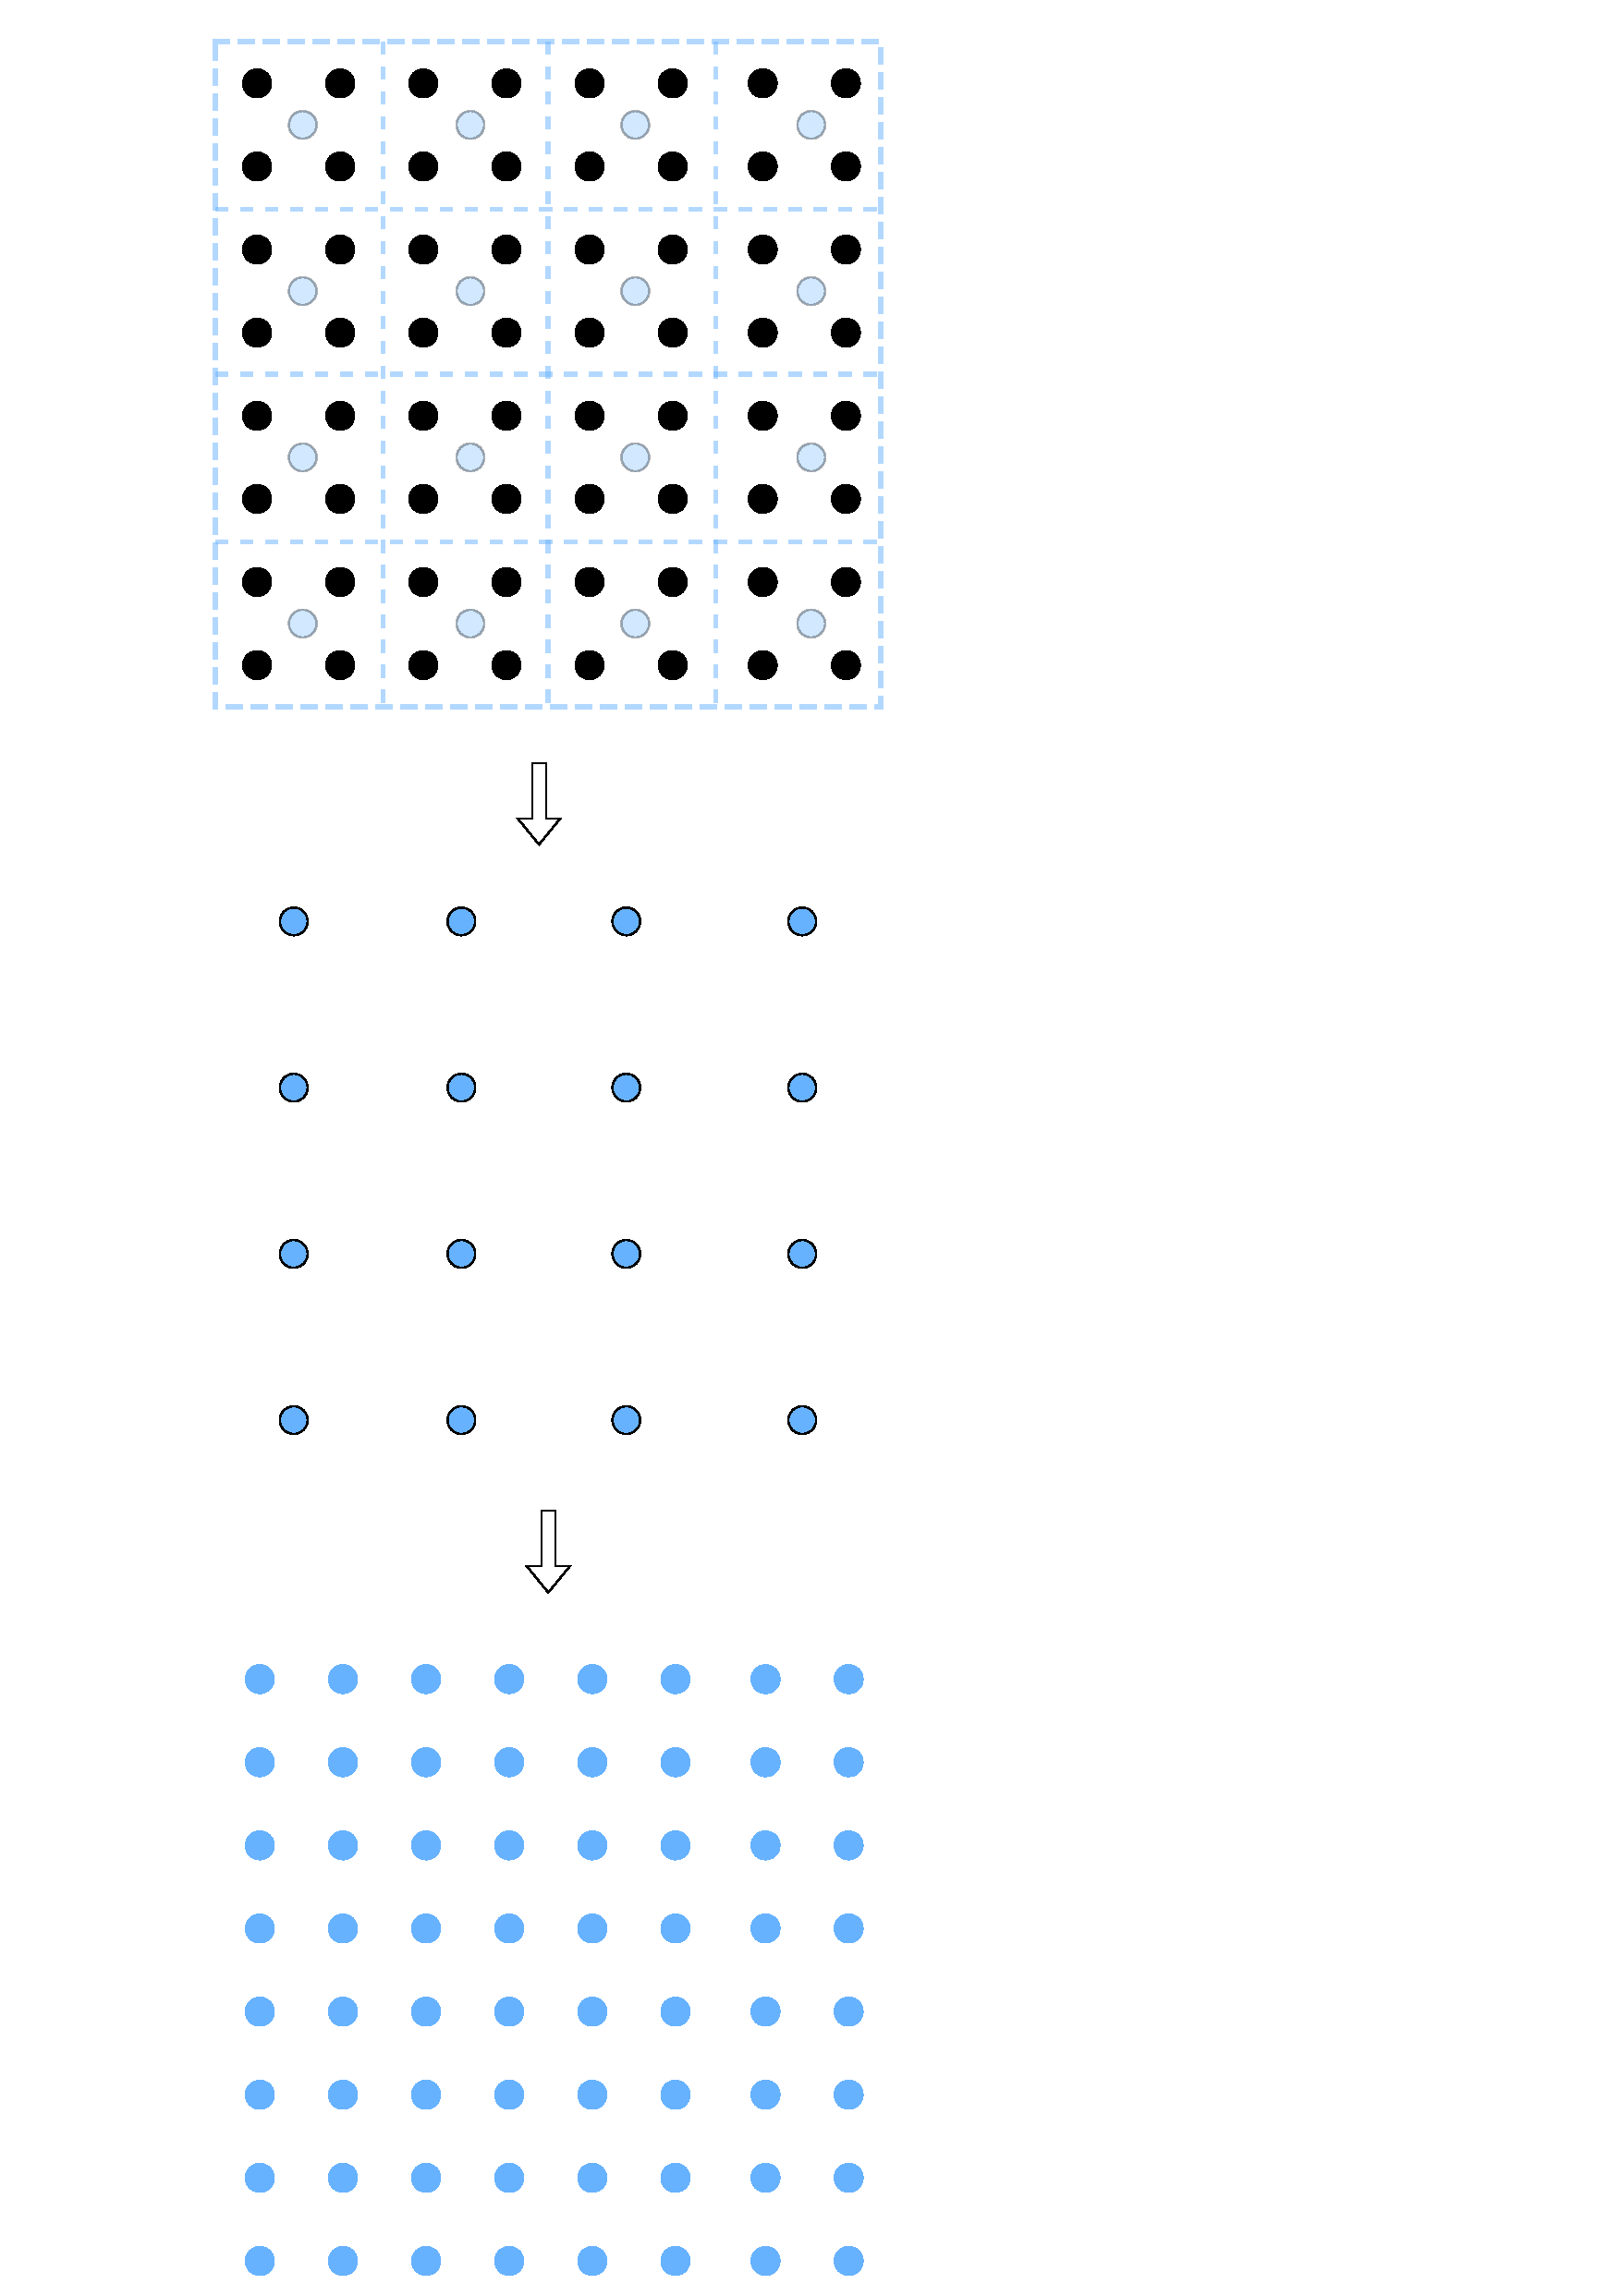
\includegraphics[angle=90,scale=0.34]{figures/test.pdf}
    \caption{test, I was very bad at art}
    \label{fig:blockin_first}
\end{figure}
Landau's mean field approach to study phase transition \cite{Landau:1937obd} gained wide popularity in the 1930's and 40's, since it was able to describe critical properties of many systems and it provided inspiration for the later Landau-Ginzburg theory of superconductivity \cite{ginzburg}. Thus, it has soon proved to be inaccurate to predict some experimentally well proven properties of certain systems near their critical point \cite{Cao:1999pw}. This is because, beeing a mean field theory, it did not take into account the role of spatial fluctuations.
The idea of block-spin transformation, systematically developed by Kadanoff \cite{PhysicsPhysiqueFizika_2_263}, made a big step towards a deeper understanding of the scaling behaviour, and posed the basis for the later work of Wilson \cite{WilsonRG1,WilsonRG2,WilsonFisher}, which still constitutes the basis for modern approaches to renormalisation in field theory and statistical physics.\\~\\
To illustrate the idea, let us consider a set of spins whose magnetisation is described by a function $\varphi(x)$. The spins are located on a discrete lattice $\mathscr{L}$, so that the function assumes values only at such sites $\varphi(x_i) = \varphi_i \neq 0 \Leftrightarrow x_i \in \mathscr{L}$. Suppose then that their interaction is described by a certain action $S[\varphi]$ and a partition function
\begin{equation*}
    Z=\sum_{\varphi} \mathrm{e}^{-S[\varphi]}.
\end{equation*}
We now want to introduce a coarse-grained (or blocked) field $\bar\varphi$ within a spacetime cell of volume $\mathcal{V}$. Such a coarse grained field can be defined, for example, as an average over the spins within the cell $\mathcal{V}$. If the spins can only be $0$ or $1$ like in a Ising model, then we might opt for a majority rule \cite{cardy_1996}.
We now want to find a new action $S_b$ such that 
\begin{equation}
    Z=\sum_{\varphi} \mathrm{e}^{-S(\varphi)}= \sum_{\bar\varphi} \mathrm{e}^{-S_b\left(\bar\varphi\right)}.
\end{equation}
We can always, in principle, build an ad-hoc action that fulfills the above condition, but it is complicated, since $S_b$ can be also be very different from $S$. For example, if the action $S[\varphi]$ contains only nearest-neighbour interactions, the new actions $S'[\phi]$ can contain higher order interactions such as nearest-to-nearest neighbour, or even more. In principle, all the terms compatible with the original symmetries are allowed. 
Thus, if the behaviour of the system is dominated by long-range properties, and the volume $\mathcal{V}$ is small enough, one can expect the functional form of the microscopic action $S$ to remain approximately the same, and one has to (eventually) only adjust the couplings. \\
The coarse-graining procedure comes with a loss of resolution since the spacing is changed $a \to 2a$. This means that the system is not anymore capable of describing physics at scales below the new spacing. Hence one can rescale distances and momenta in the new action via $a \to a/2, p \to 2p$ \textcolor{red}{connect spacing with volume}. This constitutes the second step of the block-spin transformation. The whole procedure can be thought as a zoom-out with a corresponding coarse graining, in order to describe the system in terms of the relevant scales as pictured in figure \ref{fig:blockin_first}. The procedure can be iterated multiple times, provided that the higher order interactions are either negligible or taken into account. \\

\section{Wilsonian renormalisation}
\label{sec:wilson_rg}
The wilsonian picture of renormalisation \cite{WilsonRG1,WilsonRG2} is formulated in momentum space and in general is more suitable for theories in the continuum.\\
The idea is that a physical theory comes with an intrinsic cutoff $\Lambda$, which defines up to which scale the theory is valid. This theory might not be the one
we observe directly in experiments at energy scales $\Lambda'$, which we call effective theory at scale $\Lambda'$. To see how can this happen, let us consider a theory defined by the action \eqref{eq:phi4_action} and a given cutoff $\Lambda$, and let us split the field as $\Phi = \phi + \varphi$ where $\phi$ are fields with momenta $p^2 \leq \Lambda^{\prime, \, 2}$ and $\varphi$ are fields with momenta $\Lambda^{\prime \, 2} < p^2 \leq \Lambda^2$. This allows one to rewrite the path integral as
\begin{equation*}
    Z = \int D\Phi_\Lambda \, e^{-S_\Lambda[\Phi]} = \int D\phi_{\Lambda'} \, e^{-S_{\Lambda'}[\phi]} \int D\varphi_{\Lambda', \Lambda}  \, e^{-S_{\Lambda', \Lambda}[\phi, \varphi]} = \int D\phi_{\Lambda'} \, e^{-S_{\Lambda'}^\text{eff}[\phi]},
\end{equation*}
where, in the last step, we formally performed the integral over the high-momentum field $\varphi$ and defined a new effective action $S^\text{eff}_{\Lambda'}$ as
\begin{equation*}
    S_{\Lambda'}^\text{eff}[\phi] = S_{\Lambda'}[\phi] - \log\left( \int D\varphi_{\Lambda', \Lambda}  \, e^{-S_{\Lambda', \Lambda}[\phi, \varphi]}\right) =  S_{\Lambda'}[\phi] + \delta S_{\Lambda', \Lambda}[\phi].
\end{equation*}
Note that all the steps above are exact identities. At this point, one typically tries to compute $\delta S_{\Lambda', \Lambda}$ via, e.g., Feynman diagrams \cite{Peskin:1995ev}, and then expands the result in terms of local operators of the type $O_{m,n} = \partial^m_x\phi^n_x$ with respective coefficients $g_{mn}$. In general, this will generate many terms, some of which were already present in the original action $S_\Lambda$, while some others will be new. The former can be readily absorbed in $S_{\Lambda'}[\phi]$ by a redefitinion of the couplings. 
Note that the new action is not anymore capable of describing degrees of freedom above the scale $\Lambda'$, and there is loss of resolution. As for the block-spin procedure, one can operate a dimensional rescaling in order to set the theory back at its original scale. To do this, let us now define a dimensionless parameter 
\begin{equation*}
    r^2 = \frac{\Lambda^{\prime \, 2}}{\Lambda^2}, \qquad 0 \leq r \leq 1,
\end{equation*}
and let us operating the rescaling according to
\begin{equation*}
    x \to x' = rx, \qquad p \to p' = p/r.
\end{equation*}
Combining the coarse-graining effects due to the high-modes integral and dimensional rescaling, the new action $S^\text{eff}_\Lambda$ can be written as \cite{Peskin:1995ev}
\begin{equation*} 
    \begin{aligned} 
        S^\text{eff}_\Lambda[\phi]=\int_x^\prime \frac{1}{2}\left(\partial_\mu^{\prime} \phi^{\prime}\right)^2 + \frac{m_\phi^{\prime \, 2}}{2} \phi^{\prime \, 2}  + \frac{\lambda^\prime}{4 !} \phi^{\prime \, 4}+C^{\prime}\left(\partial_\mu^{\prime} \phi^{\prime}\right)^4+D^{\prime} \phi^{\prime \, 6}+\cdots.
    \end{aligned}
\end{equation*}
Each coefficient $g^\prime$ corresponding to the local operator $O_{mn}$ is given by
\begin{equation}
    g'(r) = r^{-d_g} \ \frac{(g + \delta g)}{(1 + \Delta\phi)^{n}}.
    \label{eq:couplings_redefinition}
\end{equation}
where $d_g$ is the dimension of the coupling $g$, the factor  $r^{-d_g}$ appears because of the dimensional rescaling mentioned above, $\delta g$ is the correction term that comes from the expansion of the high-momentum integral, and $Z_\phi = 1 + \Delta\phi$ is the wavefunction renormalisation. \textcolor{red}{comment a bit on this}. \\
At this point, one can clearly see the analogy with the block-spin transformation introduced in the previous section. Performing the integral over high momenta modes can be thought as performing averages (coarse graining) over neighbours. This causes a loss of resolution which can be recovered by rescaling distances and momenta, which can be pictured as a zoom out.
Therefore the philosophy of Kadanoff and Wilson approaches, was that the blocking transformation reduces the complexity of many-body
systems by systematically reducing the number of degrees of freedom being taken into account \cite{WILSON197475},
without changing the physical content of the theory. \\~\\
Note that, beeing $r$ a continuous parameter, the transformation can also be infinitesimal. In this case, the change in the couplings due to successive iterations, gives rise to a continuous flow in parameters space, which can be described by differential equations. This is captured by the beta functions 
\begin{equation*}
    \beta_g = r \, \frac{dg'(r)}{dr}.
\end{equation*}
Fixed points are given by 
\begin{equation*}
    \beta_g = 0.
\end{equation*}
Clearly, if $\delta g / g \ll 1$, $\Delta \phi \ll 1$, equation \eqref{eq:couplings_redefinition} reduces, at lowest order, to a dimensional rescaling
\begin{equation*}
    \frac{g'}{g} \approx r^{-d_g} = \left(\frac{\Lambda^\prime}{\Lambda}\right)^{-d_g},
\end{equation*}
\textcolor{blue}{The next part might be a bit too much and I don't want to go off-topic, but I wanted to put it because it really shows that the coloured stochastic quantisation and the fRG gives the same stationary p.d.f. so it is a good motivation for the former. Maybe I can do this in Appendix? Or should I just put it aside? \\}
The existence of fixed points determine whether the limit $r \to 0$ can be taken. In this case, the resulting theory is still scale-dependent and it is described by an effective action $S^\text{eff}_\Lambda$ where all the modes with $p^2 \geq \Lambda^2$ are encoded in the couplings. \\
One can write 
\begin{equation*}
    S^\text{eff}_\Lambda[\phi] = S[\phi] + \Delta S_{\Lambda}^{(\mathrm{IR})}[\hat{\phi}],
\end{equation*}
where $\Delta S_{\Lambda}^{(\mathrm{IR})}[\hat{\phi}]$ is a regulating function which typically assumes the form
\begin{equation} 
    \Delta S_{\Lambda}^{(\mathrm{IR})}[\hat{\phi}] = \frac{1}{2} \int \frac{\mathrm{d}^d p}{(2 \pi)^d} \hat{\phi}(-p) \ \Lambda^2 \, \left(\frac{1}{r_{\Lambda}(p^2)}-1\right) \ \hat{\phi}(p),
\end{equation}
and for a sharp momentum cutoff 
\begin{equation*}
    r_{\Lambda}(p^2) = \theta\left(p^2-\Lambda^2\right).
\end{equation*}
This result will allow for a deep connection between fRG and coloured stochastic quantisation.


\section{Lattice QFT and the continuum limit}
\label{sec:lattice_continuum_}
\textcolor{red}{punteggiatura formule}. \\
Lattice Quantum Field Theory is formulated on a discrete set of spacetime points. Let us then consider a lattice $\mathscr{L}$, with spacing $a$, and $N_\mu$ points in each spacetime direction $\mu$, hence a physical length $L_\mu$.
For simplicity we restricted here to a scalar field $\phi$ and we will recall fermionic properties only when relevant, but what follows is valid also for the latter. \\ 
The action and the path integral measure are now taken over discrete quantities 
\begin{equation*}
    \begin{aligned}
	    S = \int d^dx \, \mathcal{L}(\phi(x)) \qquad &\to \qquad S = a^d \sum_{n \in \mathscr{L}} \, \mathcal{L}(\phi(n)), \\
        \prod_{x} d\phi(x) \qquad &\to  \qquad \prod_{n \in \mathscr{L}} d\phi(n),
    \end{aligned}
\end{equation*}
where $\mathcal{L}(\phi)$ is the Lagrangian density function \textcolor{red}{add citation?}.  \\
The path integral is hence
\begin{equation*}
    Z = \int \prod_n d\phi(n) \, e^{-S[\phi]}
\end{equation*}
and the probability of a field configuration $\phi$
\begin{equation}
    p(\phi) = \frac{1}{Z} \, e^{-S[\phi]}.
    \label{eq:probability_distribution_lattice}
\end{equation}
Expectation value of observables are computes as
\begin{equation}
    \expect{O(\phi)}  = \frac{1}{Z} \, \int \prod_n d\phi(n) \, O(\phi) \, e^{-S[\phi]}.
    \label{eq:expectation_value_lattice}
\end{equation}
In order to simulate a theory and perform the above sums one has to go to finite volumes and eventually impose boundary conditions. In the space directions, we take periodic conditions 
\begin{equation*}
    \begin{aligned}
        \phi(t, \vec x) &= \phi(t, \vec x + T), \\
        \psi(t, \vec x) &= \psi(t, \vec x + T).
    \end{aligned}
\end{equation*}
Instead, a finite time extent is related to the temperature of the system \cite{le_bellac_1996,rothe_LGT} via
\begin{equation*}
    \beta = 1/T = 1/L_t
\end{equation*}
and boundary conditions are chosen depending on the spin-statistic of the corresponding particles, namely periodic conditions for bosons, and anti-periodic for fermions
\begin{equation*}
    \begin{aligned}
        \phi(t, \vec x) &= \phi(t + T, \vec x) \qquad \text{bosons}, \\
        \psi(t, \vec x) &= -\psi(t + T, \vec x) \quad \text{fermions}.
    \end{aligned}
\end{equation*}
Such a formulation naturally brings a momentum cutoff $\Lambda = \pi/a$ since now all the momenta are restricted to the first Brilloune zone $p_\mu \in [-\pi/a, \pi/a]$. \\
To compute observables one relies on Monte-Carlo methods to generate field configurations, sampling the distribution \eqref{eq:probability_distribution_lattice} and convergence to the statistical value given by \eqref{eq:expectation_value_lattice} is expected for $N_\text{samp} \to \infty$. To recover the continuum results, one has to take $V \to 0, a \to \infty$ (the order matters, see for example \cite{seiler}), but this task cannot be done so straightforwardly (see for example \cite{rothe_LGT}).
Instead, continuum limits of lattice theories are intimately connected to the existence of critical points. To see why this is the case, consider the dimensionless mass gap $\hat\xi = m \, a$ of a certain theory. The quantity $\xi$ is also called correlation length and it is related to the exponential decay of correlation functions between local observables measured
at different points on the lattice as given by \textcolor{red}{add ref. eq.}\\
When taking the continuum limit we want $a \to 0$, while having a finite physical mass $m$. This implies that the correlation length $\hat \xi$ has to diverge: in the language of statistical physics, this is a second order phase transition. Of course to bring the system at its critical point, where such phase transition happens, one has to tune the bare parameters $g_0^i$ to their critical values $g_0^{i \, *}$. 
To do this, one should find the zeros of the beta functions
\begin{equation*}
    \beta_g^\text{latt} = a \frac{d}{da} g(a) \overset{!}{=} 0, \qquad a = \pi/\Lambda.
\end{equation*}
As this is quite hard task, one typically relies on some approximation schemes such as employing perturbative continuum beta functions. From this description it should be clear that the spacing $a$ should not be treated as a free parameter in the continuum limit, but rather a dynamically determined quantity that depends on the couplings of the theory. \\
Note that in the limit $a \to 0$, one has $\Lambda \to \infty$. If one's scope is to simulate an effective theory which is expected to hold only up to a scale $\Lambda_\text{phys}$, one must have $\Lambda \leq \Lambda_\text{phys}$, with a consequent lower bound on the lattice spacing $a \geq a_\text{phys} = \pi / \Lambda_\text{phys}$. \\ ~

\section{Yukawa theory}
\label{sec:Yukawa_theory}
Let us consider the Yukawa theory defined by the action
\begin{equation}
\begin{aligned}
    S[\phi,\psi,\bar\psi] &= S_\phi[\phi] + S_\psi[\psi, \bar\psi] + S_\text{int}[\phi, \psi, \bar\psi]\\
     S_\phi[\phi] &= \int_x \phi_x \left(-\frac{\partial^2_x}{2} + \frac{m_\phi^2}{2}\right) \phi_x + \frac{\lambda}{4!} \, \phi_x^4 \\
     S_\psi[\psi, \bar\psi] &= \int_x \sum_{f=1}^{N_f} \bar \psi_x^{(f)} \left(\slashed{\partial}_x + m_q \right) \psi_x^{(f)} \\
     S_\text{int}[\phi, \psi, \bar\psi] &= \int_x \sum_{f=1}^{N_f} g \, \bar \psi_x^{(f)} \, \phi_x \, \psi_x^{(f)}
    \label{eq:full_action_continuum}
\end{aligned}
\end{equation}
One can see that the action is made of a scalar part $S_\phi[\phi]$, a fermionic part $S_\psi[\psi, \bar\psi]$ and a Yukawa interaction term $S_\text{int}[\phi, \psi, \bar\psi]$. \\
It is also convenient for later purposes to define the operators $K, D$ represented in position space as 
\begin{equation}
    \begin{aligned}
        K(x, y) &=  \left(-\partial^2_x + m_\phi^2\right) \ \delta(x,y) \\
        D(x, y) &= \left(\slashed{\partial}_x + m_q + g\phi \right) \ \delta(x,y)
    \end{aligned}
    \label{eq:definition_kinetic_terms_continuum_position}
\end{equation}
and in momentum space as
\begin{equation}
    \begin{aligned}
        \widetilde{K}(p, q) &=  \int_{x,y} e^{-ipx} \left(\partial^2_x + m_\phi^2\right) \ \delta(x,y) \ e^{iqy} = \left(\frac{p^2}{2} + \frac{m_\phi^2}{2}\right) \ \delta(p,q) \\
        \widetilde{D}(p, q) &= \int_{x,y} e^{-ipx} \left(\slashed{\partial}_x + m_q + g\phi \right) \ \delta(x,y) \ e^{iqy} = \left(\slashed{p}_x + m_q + g\phi \right) \ \delta(p,q)
    \end{aligned}
    \label{eq:definition_kinetic_terms_continuum_momentum}
\end{equation}
This allows one to rewrite the action as
\begin{equation*}
    S[\phi,\psi,\bar\psi] = \int_x \frac{1}{2} \, \phi_x \, K_{xx} \, \phi_x + \frac{\lambda}{4!} \, \phi_x^4 + \sum_{f=1}^{N_f} \bar\psi_x^{(f)} \, D_{xx} \, \psi_x^{(f)}
\end{equation*}
We introduce the left-handed and right-handed spinors
\begin{equation*}
	\psi_L = (1-\gamma_5) \, \psi \qquad \psi_R = (1+\gamma_5) \, \psi
\end{equation*}
for which
\begin{equation*}
	\psi = \frac{(1-\gamma_5)}{2} \psi + \frac{(1+\gamma_5)}{2} \psi = \psi_L + \psi_R
\end{equation*}
The action written in terms of $\psi_L, \psi_R$ reads
\begin{equation}
	S = S_\phi +  \bar\psi _L D \psi_L + \bar\psi _R D \psi_R + (m_q + g\phi) \,  \left(\bar\psi_L\psi_R + \bar\psi_R\psi_L\right)
	\label{eq:action_chirality_explicit}
\end{equation}
The last equation makes clear that that for $m=0,\left\langle\phi\right\rangle = 0$ the action is symmetric under the chiral group $SU(2) _L\times SU(2)_R$, namely
\begin{equation*}
	\begin{aligned}
		\psi_L(x) \to U_L\psi_L(x) &\qquad \bar\psi_L(x) \to \bar\psi_L(x) U_L^{\dagger} \\
		 \psi_R(x) \to U_R\psi_R(x) &\qquad \bar\psi_R(x) \to \bar\psi_R(x) U_R^{\dagger}
	\end{aligned}
\end{equation*}
for $U_L, U_R \in SU(2)$.\\
The main feature of the model is chiral symmetry breaking \cite{Nambu1961DynamicalI, Nambu1961DynamicalII}, which can happen explicitly at the level of the classical action for a non-zero quark mass, or spontaneously when the scalar field gains a non-zero expectation value. One can in fact notice already by looking at \eqref{eq:definition_kinetic_terms_continuum}, that $\left\langle\phi\right\rangle \neq 0$ has the same effect on the action as a finite bare quark mass. This observation will be made more quantitative in section (SECCCC) where it will be shown that  
\begin{equation*}
    \left\langle \phi \right\rangle \sim \left\langle \bar \psi \psi \right\rangle \sim m_q
\end{equation*}
The fermionic part of the path integral \eqref{eq:path_integral_generic} can be performed explicitly
\begin{equation*}
    \int \mathcal{D} \bar\psi \mathcal{D} \psi \ \exp\left( - \int_x \sum_{f=1}^{N_f} \bar\psi_x^{(f)} \,  D \, \psi_x^{(f)} \right) = (\text{det} \, D[\phi])^{N_f} = e^{N_f\tr \log (D[\phi])}
\end{equation*}
where the trace is performed over spacetime and spinor components. \\ 
The full path integral can now be expressed in terms of the resulting effective action for the scalar fields
\begin{equation*}
    Z = \int \mathcal{D}\phi \ e^{-S_\text{eff}[phi]}
\end{equation*}
with
\begin{equation}
    S_\text{eff}[\phi] = S_{\phi}[\phi] - \underset{x,s,f}{\tr} \log D[\phi]
    \label{eq:effective_action_no_fermions}
\end{equation}
One can derive the classical equations of motion by imposing $\frac{\delta S}{\delta \phi} = 0$, here expressed in momentum space
\begin{equation*}
     (k^2 + m_\phi^2) \, \phi(x) + \frac{\lambda}{6} \, \phi^3(x) = g \ \underset{s,f}{\tr} \left[D^{-1}(\phi(x)\right] = - g \ \bar\psi(x) \psi(x)
\end{equation*}
where the trace is performed over spin and flavour components. For $\lambda = 0$, they highlight a simple proportionality relation between magnetisation and chiral condensate, which for zero momentum reads
\begin{equation}
    \phi(x) = - \frac{g}{m_\phi^2} \ \bar \psi(x) \psi(x)
    \label{eq:classical_EOM}
\end{equation}
The classical relation \eqref{eq:classical_EOM} is proven to hold also at mean field on the quantum level \cite{Buballa2005NJL-modelMatter} and will be studied in the discretised theory in section \ref{sec:classical_to_quantum}. \\~\\


\begin{figure}[h]
\centering
\begin{minipage}{0.45\textwidth}
    \begin{tikzpicture}
        \begin{axis} [axis lines=center, xtick=\empty, ytick=\empty, xlabel=$\phi$, ylabel=$V(\phi)$,
        every axis x label/.style={
            at={(ticklabel* cs:1.0)},
            anchor=west,
        },
        every axis y label/.style={
            at={(ticklabel* cs:1.0)},
            anchor=south,
        },]
            \addplot [domain=-3:3, smooth, thick] { 6*x^2 + x^4 - 6*x };
        \end{axis}
     
    \end{tikzpicture}
    
\end{minipage}
\hfill
\begin{minipage}{0.45\textwidth}
    \begin{tikzpicture}
        \begin{axis} [axis lines=center, xtick=\empty, ytick=\empty, xlabel=$\phi$, ylabel=$V(\phi)$,
        every axis x label/.style={
            at={(ticklabel* cs:1.0)},
            anchor=west,
        },
        every axis y label/.style={
            at={(ticklabel* cs:1.0)},
            anchor=south,
        },]
            \addplot [domain=-3:3, smooth, thick] { -6*x^2 + x^4 - 2*x };
        \end{axis}
     
    \end{tikzpicture}
\end{minipage}
\label{fig:breaking_O1_symmetry}
\caption{The introduction of the boson-fermion interaction, with a finite fermionic mass, causes the breaking of the O(1) symmetry. It shifts the equilibrium position in the symmetric phase (left) causing $\left\langle \phi \right\rangle \neq 0$, and tilts the potential in the broken phase (right), making the two minima not equivalent.}
\end{figure}


\newpage
